\documentclass[c,unicode,russian]{beamer}
\usepackage{hyperref}
\usepackage{alltt}
\usepackage{verbatim}
\usepackage{fancyvrb}

\usepackage{fontspec}
\setsansfont{Ubuntu}
\setmonofont{Ubuntu Mono}
\usepackage{polyglossia}
\setdefaultlanguage{russian}

\useinnertheme{metropolis}
\useoutertheme{metropolis}
\usecolortheme{metropolis}

\usepackage{listings}   % C++ code
\usepackage{xcolor}     % C++ code
\lstset{%
    keywordstyle=\color{blue},
    commentstyle=\color[rgb]{0.13,0.54,0.13},
    backgroundcolor=\color{yellow!10},
    basicstyle=\small\tt,
    stringstyle=\color{red}\ttfamily,
    belowcaptionskip=-1pt,
    xleftmargin=-15pt,
    framexleftmargin=-15pt,
    framexrightmargin=5pt,
    framextopmargin=5pt,
    framexbottommargin=5pt,
    framesep=0pt,
    rulesep=0pt
}
\lstdefinestyle{cpp}{%
    language=C++,
    morecomment=[l][\color{magenta}]{\#}
}
\lstdefinestyle{python}{%
    language=Python
}

\usepackage{caption}
\renewcommand{\lstlistingname}{Код} % Listing -> Algorithm
\DeclareCaptionFont{white}{\color{white}}
\DeclareCaptionFormat{listing}{\colorbox{gray}{\parbox{\textwidth}{#1#2#3}}}
\captionsetup[lstlisting]{format=listing,labelfont=white,textfont=white}

% logo of my university
\titlegraphic{\hspace{-1cm}
\includegraphics[width=2.5in]{../../_static/logo.jpg}}

\date{}
\author{Основы Веб-программирования}
\institute{Кафедра Интеллектуальных Информационных Технологий, ИнФО, УрФУ}

\usepackage{array}      % Table

\title{WSGI}

\begin{document}

% Slide #1
\frame{\titlepage}

% Slide #2
\begin{frame}{Ресурсы}
    \url{https://en.wikipedia.org/wiki/Web_Server_Gateway_Interface}\newline
    \url{http://lectureswww.readthedocs.org/5.web.server/wsgi.html}
\end{frame}

% Slide #3
\begin{frame}{WSGI - это\ldots?}

    \textbf{Python}\newline
    \textbf{pep-333}\newline
    \textbf{pep-3333}\newline

    Спецификация простого и универсального интерфейса между Веб-сервером,
    веб-приложением или Веб-фреймворком.

\end{frame}

% Slide #4
\begin{frame}{Кто использует?}

    \textbf{Все кто на Питоне}

    BlueBream, bobo, Bottle, CherryPy, Django, Eventlet, Flask, Gevent-FastCGI,
    Google App Engine's webapp2, Gunicorn, prestans, mod\_wsgi, netius, pycnic,
    Pylons, Pyramid, restlite, Tornado, Trac, TurboGears, Uliweb, uWSGI,
    web.py, Falcon, web2py, weblayer, Werkzeug.

\end{frame}

% Slide #5
\begin{frame}{Аналоги}

    \textbf{Ruby Rack}\newline

    \url{http://rack.github.io}

\end{frame}

% Slide #6
\begin{frame}{Что даёт?}

    \begin{itemize}
        \item Соединять различные веб-сервера и приложения между
            собой, как конструктор.
        \item Добавлять между ними независимые программы
            (middleware) которые расширяют функционал.
    \end{itemize}

\end{frame}

% Slide #7
\begin{frame}{Состоит из}

    \begin{itemize}
        \item \textbf{Application}
        \item \textbf{Server}
        \item \textbf{Middleware}
    \end{itemize}

\end{frame}

% Slide #8
\begin{frame}{WSGI в действии}

    \begin{center}
        \vspace{-0.35in}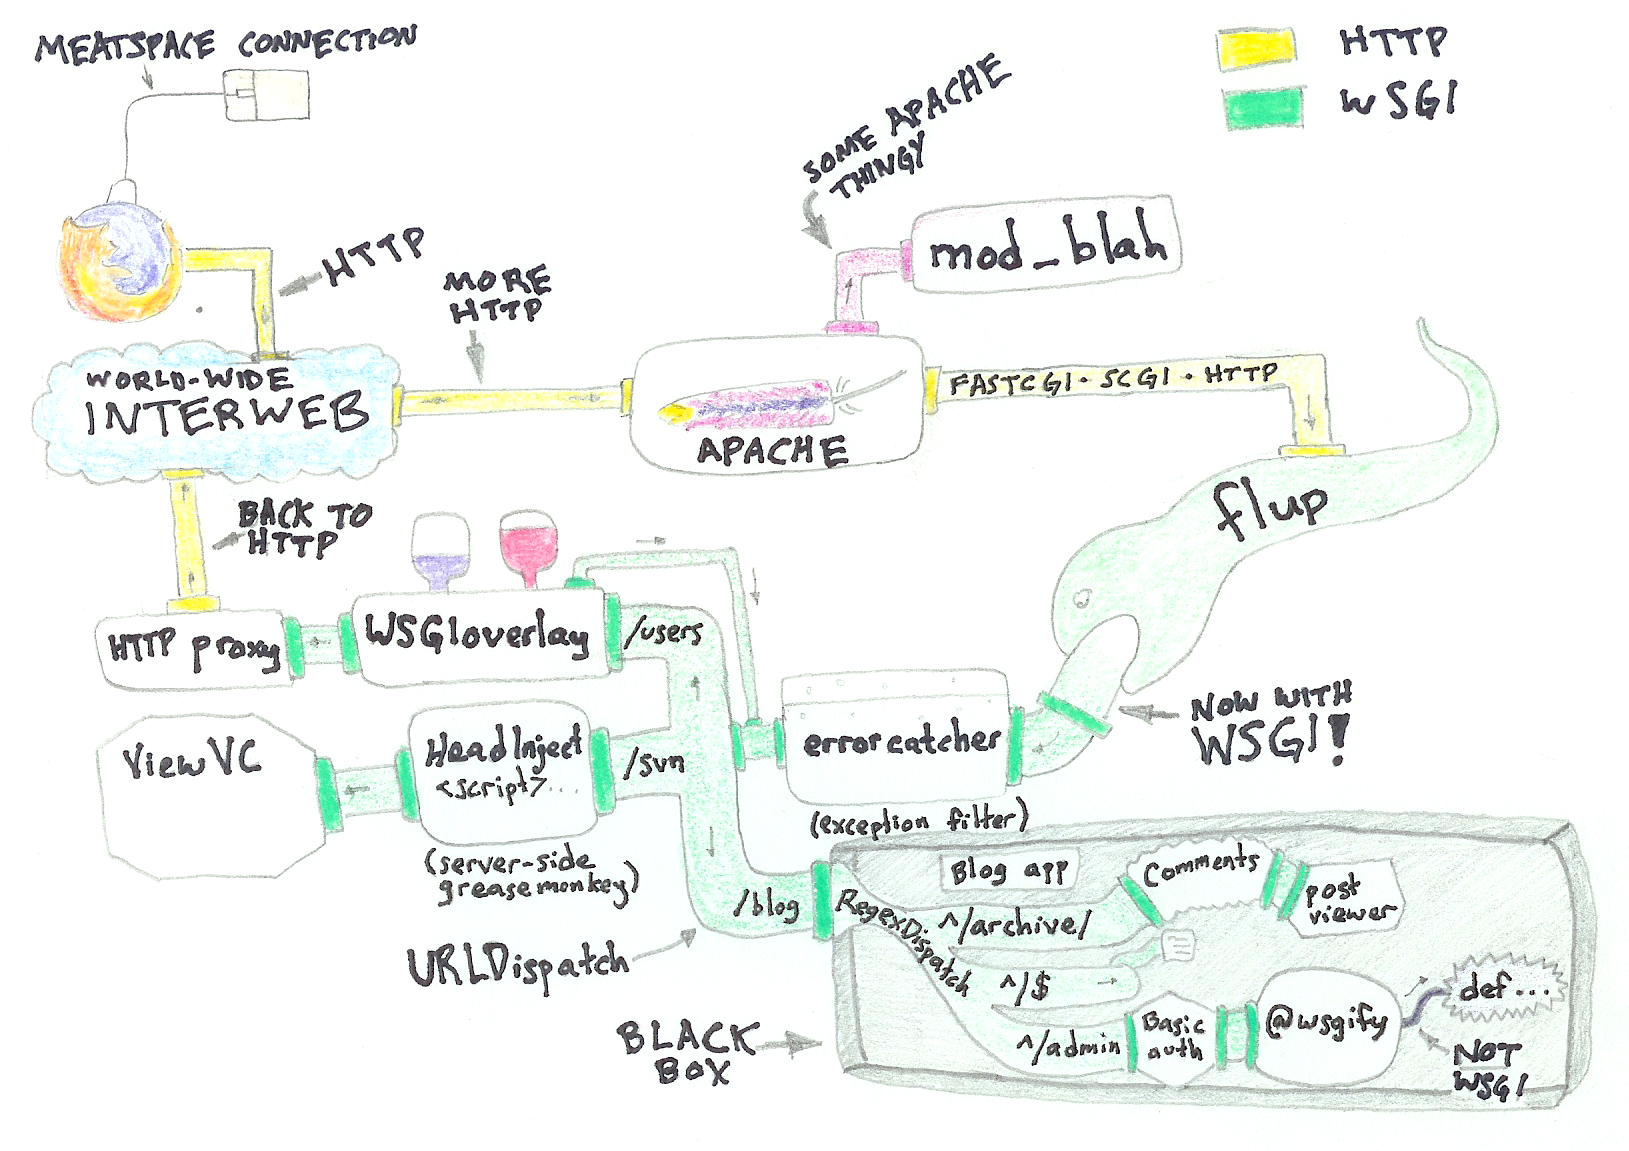
\includegraphics[width=4.4in]{media/wsgi_ianb.png}
    \end{center}

\end{frame}

% Slide #9
\begin{frame}{Application}

    \begin{itemize}
        \item должно быть вызываемым (\textbf{callable}) объектом (обычно это
            функция или метод)
        \item принимать два параметра:
            \begin{itemize}
                \item словарь переменных окружения (\textbf{environ})
                \item обработчик запроса (\textbf{start\_response})
            \end{itemize}
        \item вызывать обработчик запроса с кодом HTTP-ответа и
            HTTP-заголовками
        \item возвращать итерируемый объект с телом ответа
    \end{itemize}

\end{frame}

% Slide #10
\begin{frame}{Application}

    \begin{center}
        \vspace{-0.35in}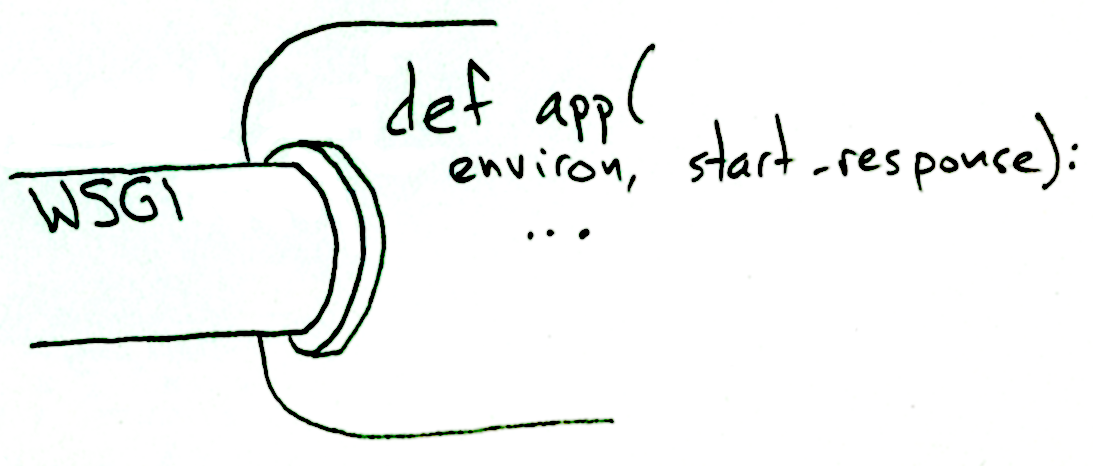
\includegraphics[width=3in]{media/wsgi-app.png}
    \end{center}

\end{frame}

% Slide #11
\begin{frame}[fragile]{Application. Функция}

    \vspace{-1in}
    \begin{lstlisting}[style=python, caption=simple WSGI application]
    def simple_app(environ, start_response):
        status = '200 OK'
        response_headers = [
            ('Content-type', 'text/plain')
        ]
        start_response(status, response_headers)
        return ['Hello world!\n']
    \end{lstlisting}

\end{frame}

% Slide #12
\begin{frame}[fragile]{Application. Класс}

    \begin{lstlisting}[style=python, caption=WSGI app class]
    class AppClass(object):
        def __init__(self, environ, start_response):
            self.environ = environ
            self.start = start_response

        def __iter__(self):
            status = '200 OK'
            response_headers = [
                ('Content-type', 'text/plain')
            ]
            self.start(status, response_headers)
            yield "Hello world!\n"
    \end{lstlisting}

\end{frame}

% Slide #13
\begin{frame}{Server}

    \begin{center}
        \vspace{-0.35in}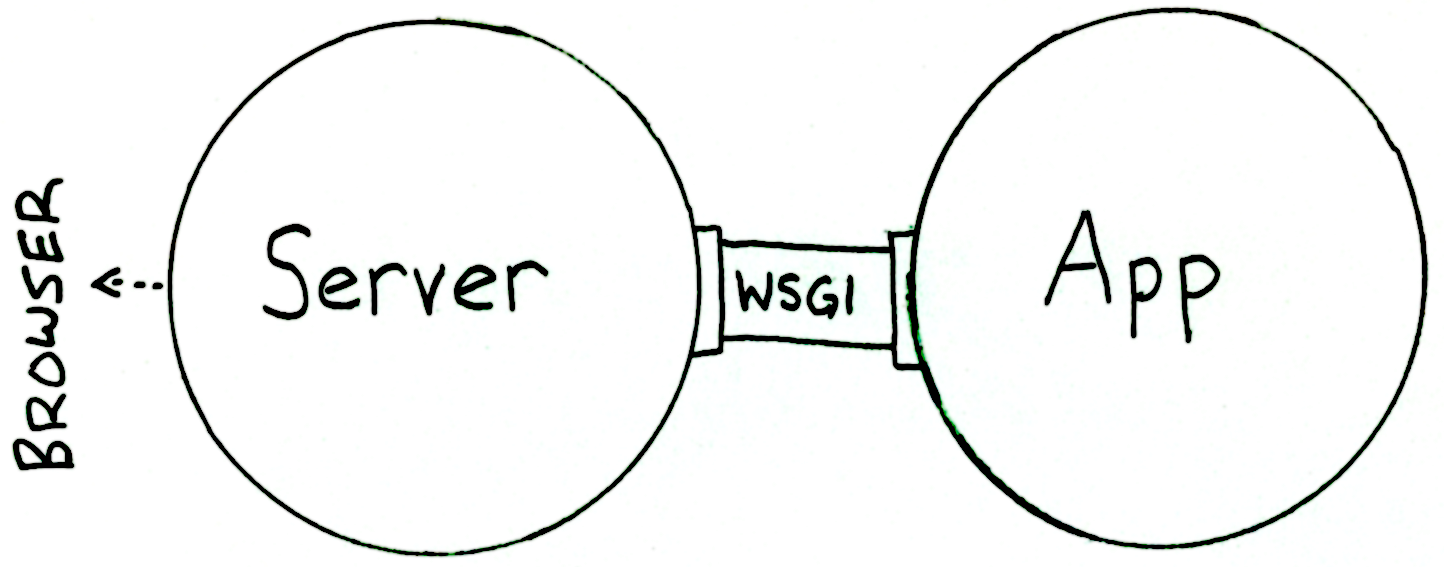
\includegraphics[width=3in]{media/server-app.png}
    \end{center}

\end{frame}

% Slide #14
\begin{frame}{Server. Задачи WSGI сервера}

    \begin{itemize}
        \item Сформировать переменные окружения (\textbf{environment})
        \item Описать функцию обработчик запроса (\textbf{start\_response})
        \item Передать их в \textbf{WSGI приложение}
        \item Результат ответа \textbf{WSGI} приложения \textbf{WSGI сервер}
          отправляет по HTTP, клиенту
    \end{itemize}

\end{frame}

% Slide #14
\begin{frame}{Server. WSGI шлюз}

    \begin{itemize}

      \item Либо \textbf{WSGI сервер} (шлюз) отправлет результат ответа proxy-серверу
        по протоколу (CGI, FastCGI, SCGI, uWSGI, \ldots), который передает его
        клиенту.
      \item Proxy сервера могут быть например \textbf{Nginx}, \textbf{Apache},
        \ldots

    \end{itemize}

\end{frame}


% Slide #14
\begin{frame}{Server. Что выбрать?}

    \begin{itemize}

      \item Waitress
      \item Gunicorn
      \item uWSGI
      \item wsgiref

    \end{itemize}

\end{frame}


% Slide #15
\begin{frame}[fragile]{Server. Написать самому}

    \begin{lstlisting}[style=python]
    def run_with_cgi(application):

        environ = dict(os.environ.items())
        environ['wsgi.input']        = sys.stdin
        environ['wsgi.errors']       = sys.stderr
        environ['wsgi.version']      = (1, 0)
        environ['wsgi.multithread']  = False
        environ['wsgi.multiprocess'] = True
        environ['wsgi.run_once']     = True

        if environ.get('HTTPS', 'off') in ('on', '1'):
            environ['wsgi.url_scheme'] = 'https'
        else:
            environ['wsgi.url_scheme'] = 'http'
    \end{lstlisting}

\end{frame}

% Slide #16
\begin{frame}[fragile]{Server}

    \begin{lstlisting}[style=python]
    headers_set = []
    headers_sent = []

    def write(data):
     if not headers_set:
       raise Exception("write() before start_response")
     elif not headers_sent:
       # Before the first output, send the stored headers
       status, response_headers = headers_sent[:] \
         = headers_set
       sys.stdout.write('Status: %s\r\n' % status)
       for header in response_headers:
         sys.stdout.write('%s: %s\r\n' % header)
         sys.stdout.write('\r\n')
     sys.stdout.write(data)
     sys.stdout.flush()
    \end{lstlisting}

\end{frame}

% Slide #17
\begin{frame}[fragile]{Server}

    \begin{lstlisting}[style=python]
    def start_response(status, response_headers, exc_info=None):
      if exc_info:
        try:
          if headers_sent:
            # Re-raise original exception if headers sent
            raise Exception(exc_info[0], exc_info[1], exc_info[2])
        finally:
          exc_info = None  # avoid dangling circular ref
      elif headers_set:
        raise AssertionError("Headers already set!")
      headers_set[:] = [status, response_headers]
      return write
    \end{lstlisting}

\end{frame}

% Slide #18
\begin{frame}[fragile]{Server}

    \begin{lstlisting}[style=python]
    result = application(environ, start_response)
    try:
      for data in result:
        if data:  # don't send headers until body appears
          write(data)
      if not headers_sent:
        write('')  # send headers now if body was empty
    finally:
      if hasattr(result, 'close'):
        result.close()
    \end{lstlisting}

\end{frame}

% Slide #19
\begin{frame}[fragile]{Запуск WSGI приложения}

    \begin{lstlisting}[style=python]
    run_with_cgi(simple_app)
    \end{lstlisting}

    \begin{lstlisting}[style=python]
    $ python 1.cgi.app.py
    Status: 200 OK
    Content-type: text/plain

    Hello world!
    \end{lstlisting}

\end{frame}

% Slide #20
\begin{frame}{Middleware}

    То есть для сервера \textbf{middleware} является приложением, а для
    приложения — сервером.

    Это позволяет составлять «цепочки» WSGI-совместимых \textbf{middleware}.

\end{frame}

% Slide #21
\begin{frame}{Middleware}

    \begin{itemize}
        \item обработка сессий
        \item аутентификация/авторизация
        \item управление URL (маршрутизация запросов)
        \item балансировка нагрузки
        \item пост-обработка выходных данных (например, проверка на валидность)
        \item и прочее \ldots
    \end{itemize}

\end{frame}

% Slide #30
\begin{frame}[fragile]{Middleware. Все вместе}
    \begin{lstlisting}[style=python]
    app = EvalException(app)   # go to /Errors
    app = SessionMiddleware(app)
    app = GzipMiddleware(app)
    app = PonyMiddleware(app)  # go to /pony

    from paste.httpserver import serve
    serve(app, host='0.0.0.0', port=8000)
    \end{lstlisting}
\end{frame}

% Slide #22
\begin{frame}{Middleware. Application}

    \begin{center}
        \vspace{-0.35in}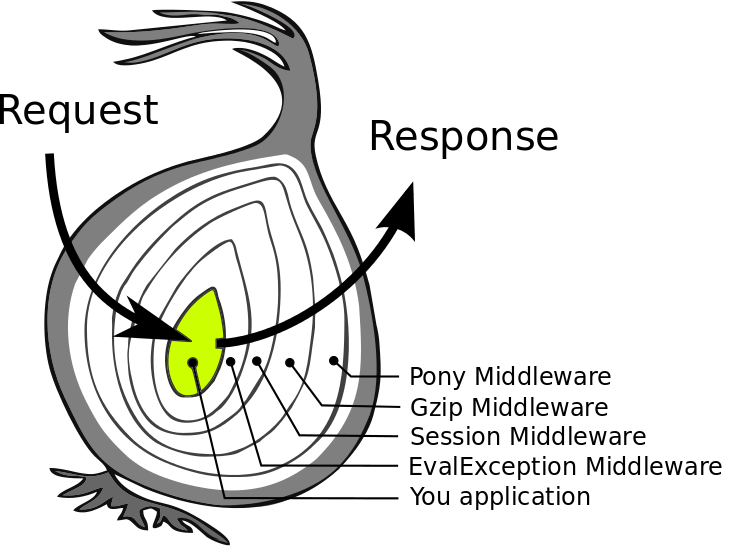
\includegraphics[width=3in]{media/wsgi-as-onion-app.png}
    \end{center}

\end{frame}

% Slide #23
\begin{frame}[fragile]{Middleware. Обработчик исключений}
    \begin{lstlisting}[style=python]
    from paste.evalexception.middleware \
        import EvalException
    app = EvalException(app)
    \end{lstlisting}
    \begin{center}
        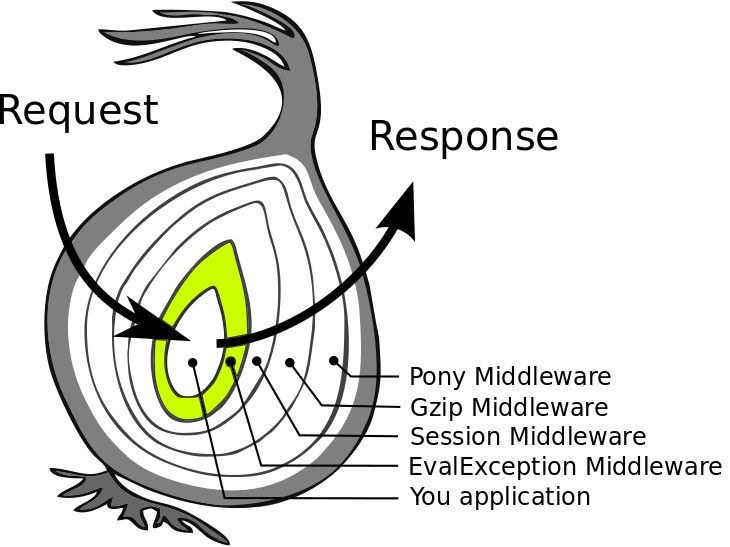
\includegraphics[width=3in]{media/wsgi-as-onion-evalexception.png}
    \end{center}
\end{frame}

% Slide #24
\begin{frame}{Middleware. Обработчик исключений}
    \begin{center}
        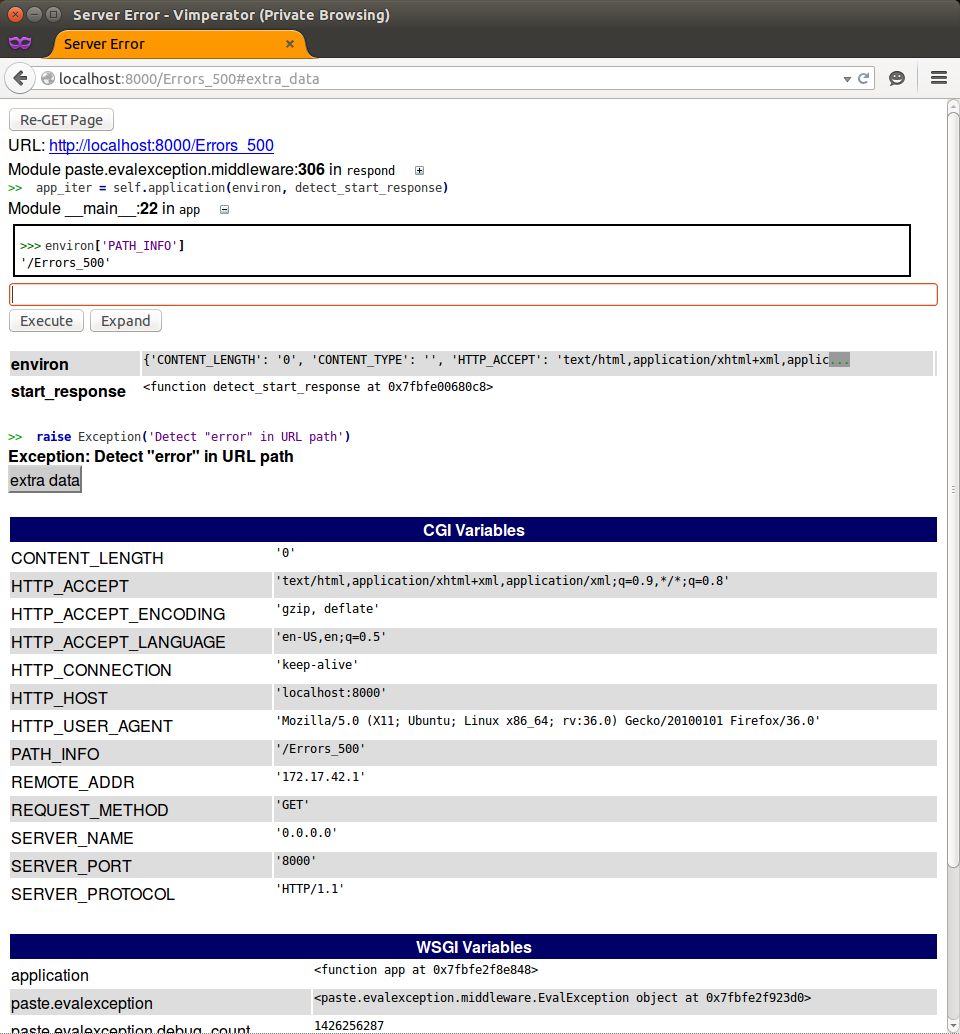
\includegraphics[width=3in]{media/wsgi_example_error.png}
    \end{center}
\end{frame}

% Slide #25
\begin{frame}[fragile]{Middleware. Сессии}
    \begin{lstlisting}[style=python]
    from paste.session import SessionMiddleware
    app = SessionMiddleware(app)
    \end{lstlisting}
    \begin{center}
        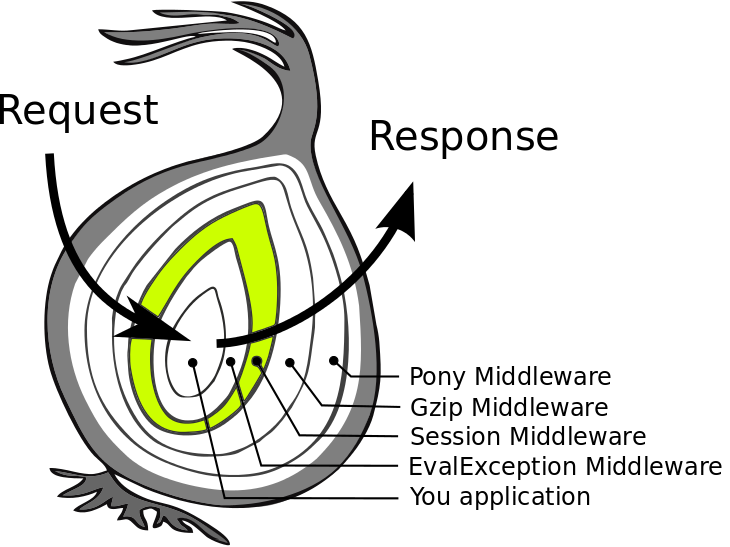
\includegraphics[width=3in]{media/wsgi_as_onion_session.png}
    \end{center}
\end{frame}

% Slide #26
\begin{frame}[fragile]{Middleware. Сжатие Gzip}
    \begin{lstlisting}[style=python]
    from paste.gzipper \
        import middleware as GzipMiddleware
    app = GzipMiddleware(app)
    \end{lstlisting}
    \begin{center}
        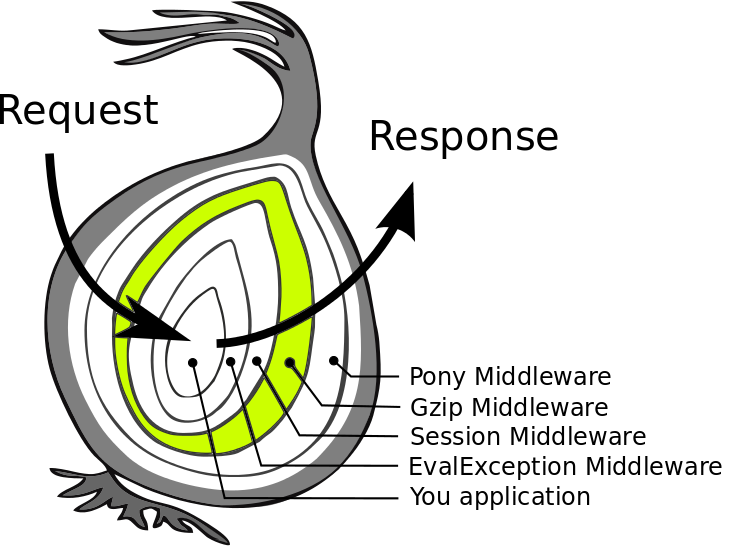
\includegraphics[width=3in]{media/wsgi_as_onion_gzip.png}
    \end{center}
\end{frame}

% Slide #27
\begin{frame}{Middleware. Сжатие Gzip}
    \begin{center}
        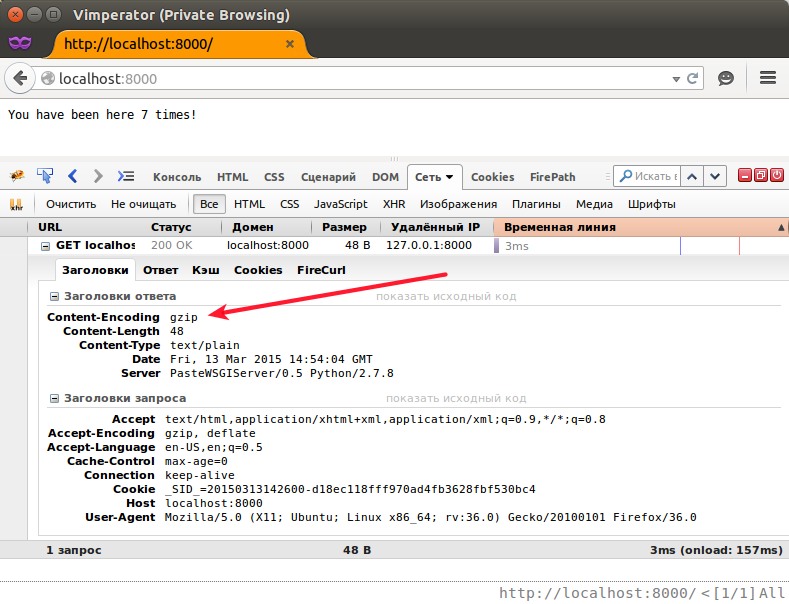
\includegraphics[width=3in]{media/wsgi_example_gzip.png}
    \end{center}
\end{frame}

% Slide #28
\begin{frame}[fragile]{Middleware. Pony}
    \begin{lstlisting}[style=python]
    from paste.pony import PonyMiddleware
    app = PonyMiddleware(app)
    \end{lstlisting}
    \begin{center}
        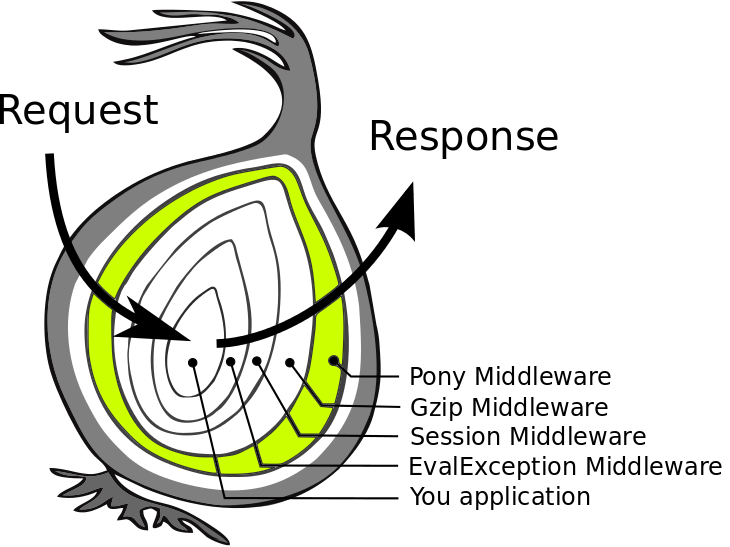
\includegraphics[width=3in]{media/wsgi_as_onion_pony.png}
    \end{center}
\end{frame}

% Slide #29
\begin{frame}{Middleware. Pony}
    \begin{center}
        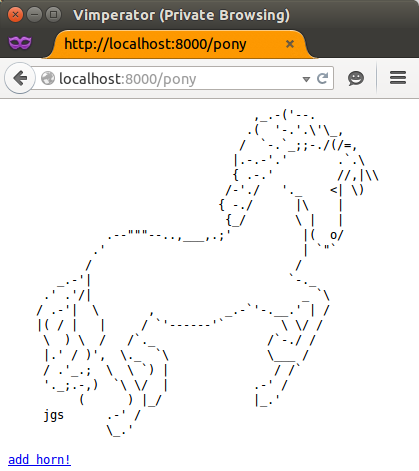
\includegraphics[width=3in]{media/wsgi_example_pony.png}
    \end{center}
\end{frame}

% Slide #31
\begin{frame}[fragile]{Middleware. Пример}
    \begin{lstlisting}[style=python]
    class GoogleRefMiddleware(object):
      def __init__(self, app):
        self.app = app

      def __call__(self, environ, start_response):
        environ['google'] = False
        if 'HTTP_REFERER' in environ:
          if environ['HTTP_REFERER']\
                .startswith('http://google.com'):
            environ['google'] = True
        return self.app(environ, start_response)

    app = GoogleRefMiddleware(app)
    \end{lstlisting}
\end{frame}

\end{document}
